% v2-acmtog-sample.tex, dated March 7 2012
% This is a sample file for ACM Transactions on Graphics
%
% Compilation using 'acmtog.cls' - version 1.2 (March 2012), Aptara Inc.
% (c) 2010 Association for Computing Machinery (ACM)
%
% Questions/Suggestions/Feedback should be addressed to => "acmtexsupport@aptaracorp.com".
% Users can also go through the FAQs available on the journal's submission webpage.
%
% Steps to compile: latex, bibtex, latex latex
%
% For tracking purposes => this is v1.2 - March 2012
\documentclass{acmtog} % V1.2

\acmYear{2019}
\acmMonth{January}

\begin{document}

\markboth{Feixiang Xu and Hengkui Cao}{Classification of Academic Topics Based on LDA}

\title{Classification of Academic Topics\\ Based on LDA} % title

\author{516030910536 Feixiang Xu \\ 516030910520 Hengkui Cao
\affil{Shanghai Jiaotong University}}


\maketitle

\begin{abstract}
Abstract: We studied and applied supervised latent Dirichlet allocation (sLDA), a statistical topic model of labelled documents. We use sLDA on our real-world problem: classification of Chinese academic topics. We adopt approximate maximum-likelihood procedure for parameter estimation, and then we use the fitted model to predict response values for new academic topics. 
When applying to the Chinese classification problem, we have solved some derivative problems. We quantify the Chinese documents by converting them to vectors based on continuous bag of words. Besides, due to the limitation of direct segmentation of academic text, we tried to promote the result of the segmentation by adding fixed match of words. We discovered new academic terminology by text mining based on Hidden Markov Model (HMM).
\end{abstract}

\section{Introduction}
LDA allows us to discover connected topics and trends within topic. Unsupervised LDA has previously been used to construct features for classification. The hope was that LDA topics would turn out to be useful for categorization, since they act to reduce data dimension. However, when the goal is prediction, fitting unsupervised topics may not be a good choice. Consider predicting a movie rating from the words in its review. Intuitively, good predictive topics will differentiate words like “excellent”, “terrible”, and “average”, without regard to genre. But topics estimated from an unsupervised model may correspond to genres, if that is the dominant structure in the corpus. The distinction between unsupervised and supervised topic models is mirrored in existing dimension-reduction techniques.

In our work, there are a large number of Chinese academic topics. Each of these academic topics belongs to a specific field. Figure 1 shows some examples of the relationships between academic topics and their corresponding fields.




\begin{figure*}[h]
\centerline{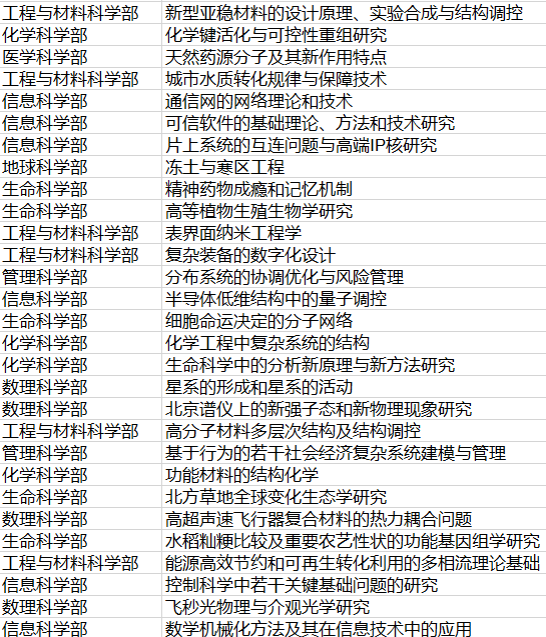
\includegraphics[width=7cm]{Figure 1.png}}
\caption{some examples of the relationships between academic topics and their corresponding fields}
  \label{fig:videocomparison}
\end{figure*}

Our goal is to train models to predict which field the new academic topics belong to, based on the existing relationships between a large number of academic topics and fields, so that automatic classification can be achieved.
In order to extract the potential information of the topics, we must first carry out Chinese word segmentation. The problem is that the word segmentation system does not recognize academic proper nouns, so that a satisfactory word segmentation effect cannot be obtained. In order to solve this problem, we use Hidden Markov Chain (HMM) to first automatically discover new academic words that are not in the word segmentation system library.
After segmentation, we have done some common treatments in the NLP field, such as removing stop words, converting Chinese words into word vectors, and building a corpus. Then get a model by training based on supervised LDA.
Finally, we tested the model with some data that was not involved in the training and got the accuracy.


\section{Motivation and Background}
\label{sec:relatedwork}
%
\looseness-1Researchers need tools to explore and browse large collections of scholarly literature. When faced with access to millions of articles in their fields, they must not be satisfied with simple search. They want interacting with the scholarly literature in a more structured way: finding articles similar to those of interest, and exploring the collection based on the underlying topics. Topic models are probabilistic models for uncovering the semantic of a document collection based on a hierarchical Bayesian analysis of the original texts.

Formally, a topic is a probability distribution over terms in a vocabulary. Informally, a topic represents an underlying semantic theme; a document consisting of a large number of words might be concisely modelled as deriving from a smaller number of topics. Such topic models provide useful descriptive statistics for a collection, which facilitates tasks like browsing, searching, and assessing document similarity. Most topic models, such as latent Dirichlet allocation (LDA), are unsupervised. Only the words in the documents are modelled, and the goal is to infer topics that maximize the likelihood (or the posterior probability) of the collection. This is compelling with only the documents as input, one can find patterns of words that reflect the broad themes that run through them and unsupervised topic modeling has many applications.


\section{Problem Formulation}
\label{sec:biologicalreview}

\subsection{Overview}

The problem can be divided into three major parts: the establishment of the terminology library, Chinese text processing, and model training based on sLDA.

\subsection{Detail}

The existing dataset contains a large number of academic topics and their one-to-one correspondence fields, we need to train a model to predict the field to which an academic topic belongs, so as to achieve automatic classification of the topics.
In our specific project, the magnitude of data is on the order of 100,000, and the number of fields is six, that is, the academic topics should be divided into six categories.


\section{Proposed Methods}
\label{sub:models_of_pupil_dynamics}

\subsection{supervised Latent Dirichlet Distribution}
LDA is a topic model, which can give the theme of each document in the document set as a probability distribution. By analyzing some documents and extracting their themes (distribution), you can make themes according to the theme (distribution). Cluster or text classification. At the same time, it is a typical word bag model, that is, a document is composed of a group of words, and there is no order relationship between words and words.In addition, a document can contain multiple topics, and each word in the document is generated by one of the topics.

LDA is about doing this: according to a given document, the theme distribution is reversed.
In the LDA model, a document is generated in the following way:
\begin{enumerate}
    \item Sampling from Dirichlet Distribution $\alpha$ to generate the subject distribution $\theta _ { i }$  of the document.
    
    \item Sampling a document from the polynomial distribution $\theta _ { i }$ of the topic i The subject of the jth word $z _ { i , j }$.
    
    \item Sampling from the Dirichlet distribution $\beta$ to generate the word distribution $\phi _ { z _ { i , j } }$  corresponding to the subject $z _ { i , j }$.
    
    \item Sampling from the polynomial distribution $\phi _ { z _ { i , j } }$ of the word and finally generating the word $z _ { i , j }$.
\end{enumerate}

Among them, the Beta-like distribution is the conjugate prior probability distribution of the binomial distribution, and the Dirichlet distribution (Dirichlet distribution) is the conjugate prior probability distribution of the polynomial distribution.

In supervised latent Dirichlet allocation (sLDA), we add to LDA a response variable connected to each document. As mentioned, examples of this variable include the number of stars given to a movie, the number of times an on-line article was downloaded, or the category of a document. We jointly model the documents and the responses, in order to find latent topics that will best predict the response variables for future unlabeled documents. sLDA uses the same probabilistic machinery as a generalized linear model to accommodate various types of response: unconstrained real values, real values constrained to be positive (e.g., failure times), ordered or unordered class labels, non-negative integers (e.g., count data), and other types.

\begin{figure*}[h]
\centerline{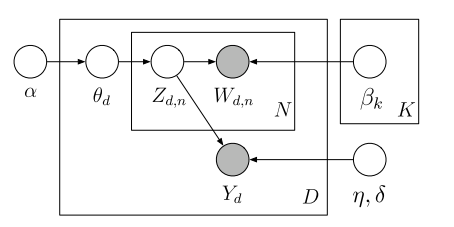
\includegraphics[width=10cm]{Figure 5.png}}
\caption{Probabilistic model diagram model of sLDA}
  \label{fig:videocomparison}
\end{figure*}

Fix for a moment the model parameters: K topics $\beta$ 1:K (each $\beta$k a vector of term probabilities), a Dirichlet parameter $\alpha$, and response parameters $\eta$ and $\delta$. (These response parameters are described in detail below.) Under the sLDA model, each document and response arises from the following generative process:

\begin{enumerate}
    \item Draw topic proportions$\theta | \alpha \sim \operatorname { Dir } ( \alpha )$
    \item For each word, draw topic assignment$z _ { n } | \theta \sim \operatorname { Mult } ( \theta )$, then Draw word$w _ { n } \left| z _ { n } , \beta _ { 1 : K } \sim \operatorname { Mult } \left( \beta _ { z _ { n } } \right)\right.$
    \item Draw response variable$y \left| z _ { 1 : N } , \eta , \delta \sim \operatorname { GLM } ( \overline { z } , \eta , \delta )\right.$, $\overline { z } : = ( 1 / N ) \sum _ { n = 1 } ^ { N } z _ { n }$
\end{enumerate}

The distribution of the response is a generalized linear model
$p ( y | z _ { 1 : N } , \eta , \delta ) = h ( y , \delta ) \exp \left\{ \frac { \left( \eta ^ { \top } \overline { z } \right) y - A \left( \eta ^ { \top } \overline { z } \right) } { \delta } \right\}$


\subsection{HMM for New Words Discovery}
In the Chinese word segmentation of the HMM model, our input is a sentence (that is, a sequence of observations), and the output is the state value of each word in the sentence. 

HMM is a triple (pi, A, B):
Initialize probability vector:  $\Pi = \left( \pi _ { i } \right)$ 
State transition matrix:  $A = \left( a _ { i j } \right) \quad \operatorname { Pr } \left( x _ { i , } | x _ { j _ { t - 1 } } \right)$
The transition probability is a very important knowledge point of the Markov chain. People who have learned probability theory in the university know that the biggest feature of the Markov chain is the state of the current T=i state Status(i), only with T=i. Related to the n states before the moment. That is: {Status(i-1), Status(i-2), Status(i-3),...Status(i-n)}

Furthermore, the HMM model has three basic assumptions as a premise of the model, including a finite historical hypothesis, that is, n=1 of the Markov chain. That is, Status(i) is only related to Status(i-1), and this assumption can greatly simplify the problem. Looking back at the transfer matrix, it is actually a two-dimensional matrix of 4x4 (4 is the size of the state value set).In the confusion matrix, each element is actually a conditional probability. According to the three observations of the three basic assumptions of the HMM model (see the comments on the independence of observations), the observations only depend on the current state value. Is:
P(Observed[i], Status[j]) = P(Status[j]) * P(Observed[i]|Status[j]). The value of P(Observed[i]|Status[j]) is obtained from the confusion matrix.


In the new word recognition, the ternary array is linked by a viterbi algorithm, the triplet is the input, and the output is the state sequence value. With the ternary array of HMM, it is equivalent to having a certain hidden Markov model. In the new word recognition, the new word can be identified by using the viterbi algorithm.




\section{Experiment}
\label{sec:proposed_model}

\subsection{Segmentation}

At first we used the jieba library to segment the academic topics. Jieba is a mature method commonly used in Chinese word segmentation in the field of NLP. Soon we found that there was a problem with the result of the jieba segmentation. There is a lack of terminology in jieba's library, which is an important component of the academic topics. Thus the result contains many impropriate segmentation, which has an adverse effect on the results.

Thus we started to explore effective improvements. We found that jieba reserved a library for us. By artificially adding vocabulary to it, jieba will remain the integrity of the words in it when segmenting.

However, manually adding words can be a n extremely hard work, due to the large amount of the words. So we used a clever and efficient method, that is using Hidden Markov Chain (HMM) to conduct the segmentation. According to the principle of HMM segmentation we just explained, we can get a segmentation with new words been automatically discovered.

\begin{figure}[h]
\centerline{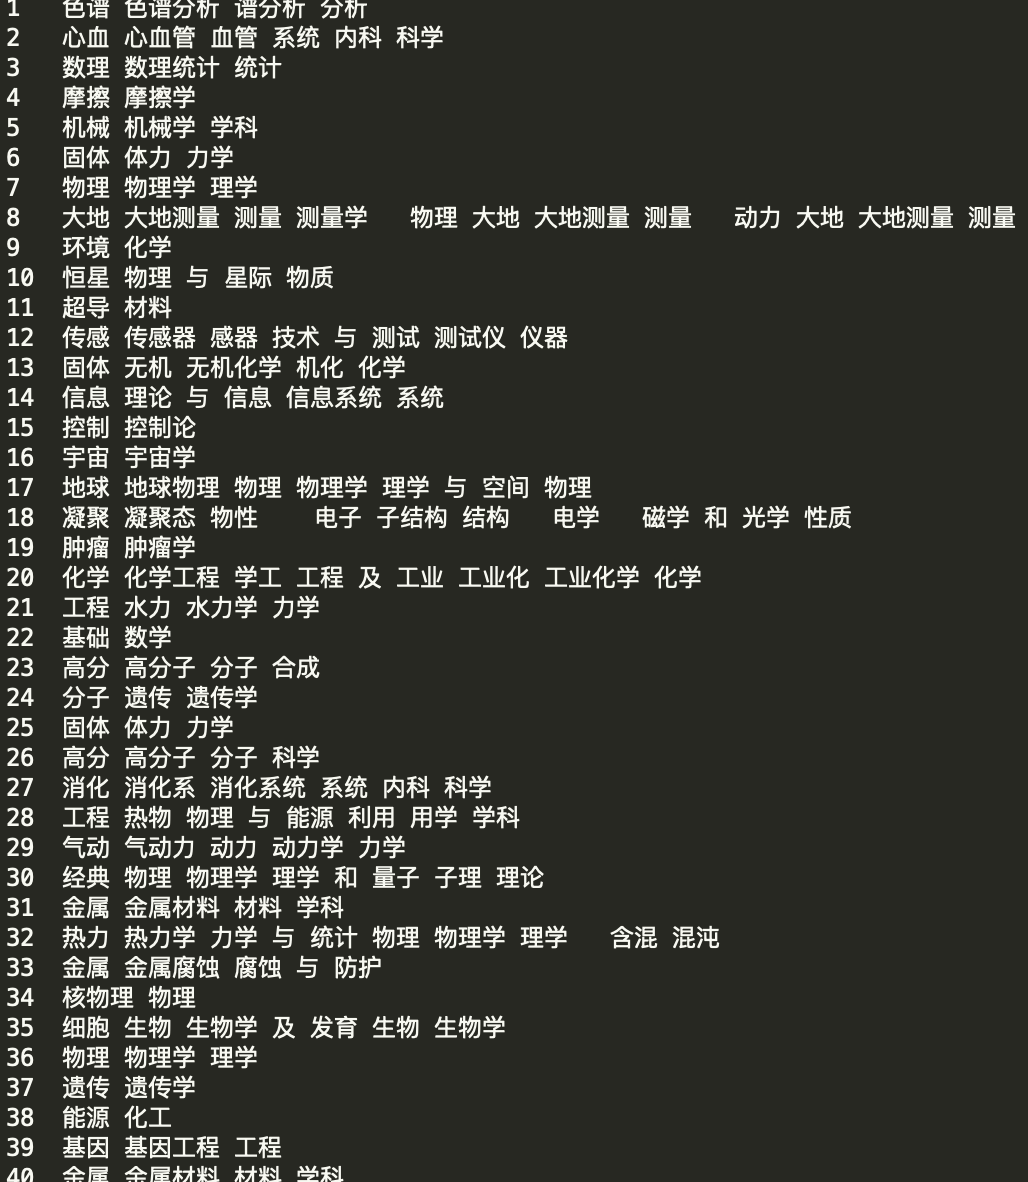
\includegraphics[width=6cm]{Figure 2.png}}
\caption{some examples of the segmentation results}
  \label{fig:videocomparison}
\end{figure}


Figure shows some examples of the segmentation. From the examples we can see that much of the terminologies have been separated out and completely retained. This indicates that the applying of HMM in segmentation does work, comparing to the directly segmentation without HMM.
Professor Jiang suggested that the IEEE Association has a list of a large number of academic vocabulary, which contains enough academic vocabulary in various fields to be used for our word segmentation. However, what we are doing is the classification of Chinese academic topics. The vast majority of the existing information is in English. It is difficult for us to find references to Chinese. Thus, we choose to find our own way to solve this problem.


\subsection{Text Processing}
\label{subsec:EquilibriumCase}
This part of work contains some common operation on Chinese text processing in NLP field. The purpose of these processes is to gradually transform the Chinese text into a mathematical expression that can be quantified.
After segmentation and the removing of stop-words, we got a satisfying segmentation result, just like the figure shows. This provides us with easy-to-use materials for our next text processing. The library gensim provides us some convenient approaches for text-vector converting. We then establish a corpus for the text, which consists of the vectors that the text has been converted to. The process of converting Chinese text to vectors is based on the calculation of TF-IDF values. TF-IDF (term frequency–inverse document frequency) is a commonly used weighting technique for information retrieval and data mining. TF means Term Frequency, and IDF means Inverse Document Frequency. TF-IDF is a statistical method used to assess the importance of a word for a file set or one of the files in a corpus. The importance of a word increases proportionally with the number of times it appears in the file, but it also decreases inversely with the frequency it appears in the corpus. The main idea is that if a word or phrase appears in an article with a high frequency and rarely appears in other articles, the word or phrase is considered to have a good class distinguishing ability and is suitable for classification.

\begin{figure}[h]
\centerline{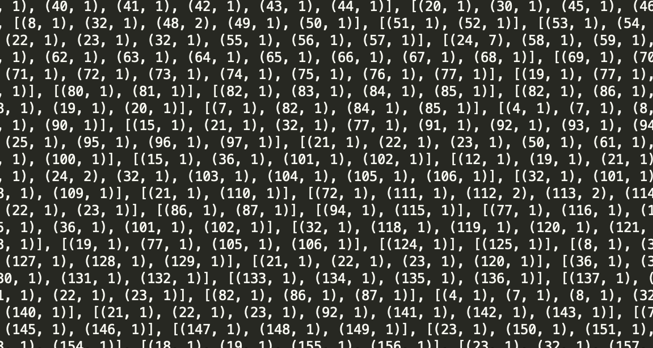
\includegraphics[width=7cm]{Figure 3.png}}
\caption{part of the corpus}
  \label{fig:videocomparison}
\end{figure}

The figure shows part of the corpus. It can be seen that the corpus is filled with the word vector, which proves that our processing work is successful. These word vectors can be used for subsequent training.

%
\subsection{Training and Testing}
\label{subsec:DynamicCase}
%
After the corpus is established, it can be trained based on the correspondence between word vectors and fields in corpus. The training is based on LDA, and the principles of LDA have been introduced earlier. In our project, the six categories to be divided into total are deterministic, so it is appropriate to use supervised learning, i.e. sLDA.
As mentioned in the introduction to the model principle, we used Gibbs Sampling for the posterior distribution of LDA. The speed of Gibbs Sampling itself is very fast, which makes the training process not take too long. Hundreds of thousands of pieces of data are trained and only used for a few minutes, which reflects the high efficiency of the LDA model in practical applications.
During training, we specifically divided some of the data as a test set, and this part of the data did not participate in the training. When the model training is completed, we apply the model to the test set and get a preliminary accuracy of 0.624, as shown in the figure.

\begin{figure}[h]
\centerline{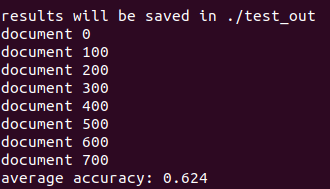
\includegraphics[width=7cm]{Figure 4.png}}
\caption{test results}
  \label{fig:videocomparison}
\end{figure}

This result indicates that the model may not be satisfactory if applied directly to the classification. However, considering that we have divided all academic topics into a total of six fields, it is understandable that the accuracy of the results is not high. In fact, this result is enough to show that it is very effective when we combining HMM, sLDA and text processing. The results of 0.624 can fully prove that the sLDA topic model does work in our real-world problem solving.

%


\section{Conclusion}
\label{sec:conclusion}
%
We studied the principle and application of supervised latent Dirichlet allocation (sLDA) and tried to apply it to solve the field-classification problem of Chinese academic topics in the real-world. In the process of dealing with Chinese academic topics, we solved the derived problems of academic terminology and the conversion of Chinese text into vectors. We uses a much effective method of discovering new words by applying Hidden Markov Chain (HMM) to improve word segmentation. We trained the processed data based on the sLDA principle and test the resulting model. The final result proved that our application of sLDA for Chinese academic topic classification is effective.

\cite{mcauliffe2008supervised}
\cite{bodrunova2013interval}
\cite{bickel2015mathematical}
\cite{blei2009topic}
\cite{yu2010hidden}
\cite{morwal2012named}

% Start of "Sample References" section


% Bibliography
\bibliographystyle{ACM-Reference-Format-Journals}
\bibliography{acmtog-sample-bibfile}
                                % Sample .bib file with references that match those in
                                % the 'Specifications Document (V1.5)' as well containing
                                % 'legacy' bibs and bibs with 'alternate codings'.
                                % Gerry Murray - March 2012

\end{document}
% End of v2-acmtog-sample.tex (March 2012) - Gerry Murray, ACM
